\documentclass[review]{elsarticle}

\usepackage{lineno,hyperref}

\usepackage{latexsym,amsthm,amsmath,amssymb,mathrsfs,dsfont,upgreek,stackengine,graphicx,caption, float,enumerate}
\usepackage{pdfpages,courier,subcaption,inputenc,tikz,verbatim,blkarray, listings,latexsym,pythonhighlight,xcolor,geometry,xparse}
\usepackage{algorithmic}
\usepackage{multirow, array, textcomp, subcaption, stmaryrd}

\newcolumntype{P}[1]{>{\centering\arraybackslash}p{#1}} % To make the data in the table be centering
\newcolumntype{M}[1]{>{\centering\arraybackslash}m{#1}}


\newcommand{\code}[1]{\colorbox{light-gray}{\texttt{#1}}}

\usepackage[ruled,vlined]{algorithm2e}


\newtheorem{remark}{Remark}
\newtheorem{theorem}{Theorem}

\modulolinenumbers[5]

\journal{Journal of Computational Physics}

\geometry{a4paper,left=2cm,right=2cm,top=1cm,bottom=1.5cm}

%%%%%%%%%%%%%%%%%%%%%%%
%% Elsevier bibliography styles
%%%%%%%%%%%%%%%%%%%%%%%
%% To change the style, put a % in front of the second line of the current style and
%% remove the % from the second line of the style you would like to use.
%%%%%%%%%%%%%%%%%%%%%%%

%% Numbered
%\bibliographystyle{model1-num-names}

%% Numbered without titles
%\bibliographystyle{model1a-num-names}

%% Harvard
%\bibliographystyle{model2-names.bst}\biboptions{authoryear}

%% Vancouver numbered
%\usepackage{numcompress}\bibliographystyle{model3-num-names}

%% Vancouver name/year
%\usepackage{numcompress}\bibliographystyle{model4-names}\biboptions{authoryear}

%% APA style
%\bibliographystyle{model5-names}\biboptions{authoryear}

%% AMA style
%\usepackage{numcompress}\bibliographystyle{model6-num-names}

%% `Elsevier LaTeX' style
\bibliographystyle{elsarticle-num}
%%%%%%%%%%%%%%%%%%%%%%%

\begin{document}

\begin{frontmatter}

\title{Numerical aspects of Casimir energy computation in acoustic scattering}
%\tnotetext[mytitlenote]{Fully 	documented templates are available in the elsarticle package on \href{http://www.ctan.org/tex-archive/macros/latex/contrib/elsarticle}{CTAN}.}

%% Group authors per affiliation:
\author[mymainaddress]{Timo Betcke}
\ead[url]{t.betcke@ucl.ac.uk}
\address[mymainaddress]{Department of Mathematics, University College London, London, WC1E 6BT, UK}


\author[mysecondaryaddress]{Alexander Strohmaier}
\ead[url]{a.strohmaier@leeds.ac.uk}
\address[mysecondaryaddress]{School of Mathematics, University of Leeds, Leeds, LS2 9JT, UK}

%% or include affiliations in footnotes:
\author[mymainaddress]{Xiaoshu Sun\corref{mycorrespondingauthor}}
\cortext[mycorrespondingauthor]{Corresponding author}
\ead[url]{xiaoshu.sun.18@ucl.ac.uk}



% \begin{abstract}
%     Computing the Casimir energy is a classical problem of quantum electrodynamics going back to the 1940s. In the early two thousands a significant breakthrough
%      was achieved by representing the Casimir energy as the computation of the integral of the log determinant of certain boundary integral operators in the complex plane. 
% Recently, this log determinant formula was investigated in the context of the Krein spectral shift function, which suggests a potential alternative computational 
% approach based on the numerical evaluation of scattering matrices. In this paper, we will give an overview of these computational techniques of computing 
% the Casimir energy in three dimensional acoustic scattering. Afterwards, we will discuss the spectral properties of the block matrices 
% inside the formula of the Casimir energy, which are constructed by the integral operators and investigate how to use these properties to speed up Casimir computations for large-scale practical problems.
% \end{abstract}

\begin{abstract}
    Computing the Casimir force and energy between objects is a classical problem of quantum theory going back to the 1940s. Several different approaches have been developed in the literature often based on different physical principles. Most notably a representation of the Casimir energy in terms of determinants of boundary layer operators makes it accessible to a numerical approach. In this paper, we first give an overview of the various methods and what is known rigorously about the connection between them. We then present a new numerical scheme for the computation of the Casimir energy for large scale problems, which is based on the spectral properties of the block matrices for the boundary layer operators. This method allows for Casimir energy calculation for large-scale practical problems and significantly speeds up the computations in that case. We also discuss the connection to the Krein-spectral shift function and computational aspects.
   \end{abstract}

\begin{keyword}
Krein spectral shift function \sep Casimir energy \sep Krylov subspace \sep inverse-free generalized eigenvalue problem \sep Bempp-cl
\end{keyword}

\end{frontmatter}

%\linenumbers
\section{Introduction}\label{Introduction}
Since late 1940s, the advanced understanding of vacuum sector of quantum electrodynamics has been developed and one of the most seminal predictions is
the vacuum effects (quantum fluctuations of the electromagnetic field) can induce attractive forces between two uncharged, perfectly conducting, parallel 
plates. This phenomenon is called \emph{Casimir effect}, which is firstly proposed by H.B.G. Casimir in 1940s \cite{casimir1948attraction}. To obtain the formula 
of the Casimir energy, he considered the space between these two plates as a type of electromagnetic cavity, solved the classical Maxwell equations with 
certain boundary condition for all the valid excitations of the electromagnetic field in this cavity and obtained countably infinite electromagnetic mode 
frequencies $\{\omega_{n}(a)\}$, where $a$ is the surface-surface distance. Accordingly, the electromagnetic zero-point energy of the $n$th cavity mode is 
$\frac{\hbar\omega_{n}(a)}{2}$ and by summing up all the contributions from the modes, he finally get the expression of the \emph{Casimir energy}:
\begin{align*}
    \mathcal{E}(a) = \frac{1}{2}\sum_{n}\hbar\omega_{n}(a),
\end{align*}
which is divergent. However, Casimir derived a finite result for the derivative of this infinite energy fluctuations, 
which is the \emph{Casimir force per unit area}:
\begin{align*}
    F(a) = -\frac{1}{A}\frac{\partial\mathcal{E}}{\partial a} = -\frac{\hbar c\pi^{2}}{240a^{4}},
\end{align*}
where $A$ is the cross-sectional area of the boundary plates. 

In 1960s, Lifshitz generalized this theory to the case of dielectric media \cite{dzyaloshinskii1961general}, which means the boundary surfaces are not perfect conductors but the real-world
materials such us the solid consisting of the atomic constituents. He proposed that any microscopic volume $\Delta V$ of the plates contains a collection of 
atomic-scale electric dipoles without uniform orientation due to the absence of the external forcing field. Once in a while, the quantum and thermal 
fluctuations may make the dipoles align spontaneously, resulting in a net electric dipole moment. It is like van der Waals interaction between the 
atoms and this dipole moment induces a net dipole field. Meanwhile, the dipoles in the opposite plate feel this field
across the gap and align as well. Now, there are two net electric dipole moments which make two plates attract with each other. Lifshitz emphasized the 
influence from the materials more than the fluctuations in the empty space between the plates and this interpretation provides little advantage on the 
computation of the Casimir energy since it is unknown on how to compute each contribution from the volume $\Delta V$. 

Afterwards, there is a decades absence of experimental input on the Casimir effect and finally in 1996, the precise measurements of the Casimir force between 
the extended bodies have been done by S.K. Lamoreaux \cite{lamoreaux1997demonstration}. From 2000 to 2008, the Casimir force has been measured in various 
experimental configurations, such as cylinder-cylinder \cite{ederth2000template}, plate-plate \cite{bressi2002measurement}, 
sphere-plate \cite{krause2007experimental} and sphere-comb \cite{chan2008measurement}. The rapid growth in experimental investigation is followed by the 
theoretical development. From 2007 to 2008, the asymptotic series of the Casimir energy have been explicitly computed in both scalar
\cite{emig2008casimir} and vector \cite{emig2007casimir} cases. In 2009, the authors of \cite{reid2009efficient} put forward a method of computing the Casimir interactions between 
arbitrary three-dimensional objects with arbitrary material properties \cite{reid2009efficient}, in which the Casimir energy between the perfectly
conducting compact objects can be described as:

\begin{align*}
    \mathcal{E} = -\frac{\hbar c}{2\pi}\int_{0}^{\infty}dk\log\frac{\mathcal{Z}(k)}{\mathcal{Z}_{\infty}(k)},
\end{align*}
where 
\begin{align}\label{functional integration}
    \mathcal{Z}(k) = \int \mathcal{D}\boldsymbol{J}(\boldsymbol{x})e^{\frac{1}{2}\int\int d\boldsymbol{x}d\boldsymbol{y}\boldsymbol{J}(\boldsymbol{x}) \cdot \boldsymbol{G}_{k}(\boldsymbol{x}, \boldsymbol{y}) \cdot \boldsymbol{J}(\boldsymbol{y})}
\end{align}
is a functional integration extending over all possible surface current distributions $\boldsymbol{J}(\boldsymbol{x})$ on the objects and 
$\mathcal{Z}_{\infty}(k)$ is $\mathcal{Z}(k)$ computed with all the objects removed to infinite separation. Moreover, in \eqref{functional integration},
\begin{align*}
    \boldsymbol{G}_{k}(\boldsymbol{x}, \boldsymbol{y}) = \left[1 + \frac{1}{k^{2}}\nabla_{\boldsymbol{x}}\otimes\nabla_{\boldsymbol{y}}\right]\frac{e^{\mathrm{i}k|\boldsymbol{x} - \boldsymbol{y}|}}{4\pi|\boldsymbol{x} - \boldsymbol{y}|}
\end{align*}
is the dyadic/tensor Green's function and $k$ is the wavenumber. Johnson proposed that one could formally apply contour integral arguments to obtain the integral 
along the imaginary axis on which the integrand is nicely behaved (non-oscillatory and exponentially decaying). In this case, the Casimir energy formula 
is rewritten as 
\begin{align}\label{rotated CasE}
    \mathcal{E} = -\frac{\hbar c}{2\pi}\int_{0}^{\infty}dk\log\frac{\mathcal{Z}(\mathrm{i}k)}{\mathcal{Z}_{\infty}(\mathrm{i}k)},
\end{align}
where 
\begin{align}
    \mathcal{Z}(\mathrm{i}k) = \int \mathcal{D}\boldsymbol{J}(\boldsymbol{x})e^{\frac{1}{2}\int\int d\boldsymbol{x}d\boldsymbol{y}\boldsymbol{J}(\boldsymbol{x}) \cdot \boldsymbol{G}_{\mathrm{i}k}(\boldsymbol{x}, \boldsymbol{y}) \cdot \boldsymbol{J}(\boldsymbol{y})}
\end{align}
and 

\begin{align*}
    \boldsymbol{G}_{\mathrm{i}k}(\boldsymbol{x}, \boldsymbol{y}) = \left[1 - \frac{1}{k^{2}}\nabla_{\boldsymbol{x}}\otimes\nabla_{\boldsymbol{y}}\right]\frac{e^{-k|\boldsymbol{x} - \boldsymbol{y}|}}{4\pi|\boldsymbol{x} - \boldsymbol{y}|}.
\end{align*}

This $ \boldsymbol{G}_{\mathrm{i}k}$ is called the Wick-rotated dyadic/tensor Green's function. One can notice that this Green's function is strongly singular 
due to the second order form ($\nabla_{\boldsymbol{x}}\otimes\nabla_{\boldsymbol{y}}$). 

%In Section \ref{Numerical methods for computing the Casimir energy}, we 
%will use the integration by parts to make the integral \eqref{rotated CasE} become a numerically computable form. Moreover, after some mathematical manipulations, 
%we can obtain the formula of the Casimir energy in terms of the integral operators, which will also be discussed in Section \ref{Numerical methods for computing the Casimir energy}.


However, a more rigorous mathematical 
derivation was recently provided by Hanisch, Strohmaier and Waters \cite{hanisch2020relative} who have shown that the natural and well-defined object is the 
integral along the imaginary axis. They also provided a mathematical framework to connect the integral to families of trace formulas and the Casimir 
energy is one of the examples. To be specific, by assuming that the objects $\Omega$ is assembled from individual objects $\Omega_{j}$, for $j = 1, \dots, N$ and 
$\partial\Omega_{j}$ are the $N$ connected components of the boundary $\partial\Omega$. Then, several self-adjoint operators on $L^{2}(\mathbb{R}^{d})$
can be defined for constructing the \emph{Birman-Krein formula} later:
\begin{itemize}
    \item The operator $\Delta$ is the Laplace operator with Dirichlet boundary conditions on $\partial\Omega$.
    \item For $j = 1, \dots, N$, the operator $\Delta_{j}$ is the Laplace operator with Dirichlet boundary conditions on $\partial\Omega_{j}$.
    \item The operator $\Delta_{0}$ is the `free' Laplace operator on $\mathbb{R}^{d}$ with domain $H^{2}(\mathbb{R}^{d})$.
\end{itemize}

Now, the Birman-Krein formula can be written as 
\begin{align}\label{B-K formula}
    \text{Tr}\left(f(\Delta^{\frac{1}{2}}) - f(\Delta_{0}^{\frac{1}{2}}) - \left(\sum_{j = 1}^{N}[f(\Delta_{j}^{\frac{1}{2}}) - f(\Delta_{0}^{\frac{1}{2}})]\right)\right)  = \int_{0}^{\infty}f'(k)\xi(k)dk,
\end{align}
where 
\begin{align*}
    \xi(k) = \frac{1}{2\pi \mathrm{i}}\log\left(\frac{\det(S(k))}{\det(S_{1,k})\cdots\det(S_{N,k})}\right)
\end{align*}
is called the \emph{relative Krein spectral shift function} (KSSF). Here, $S_{j,k}$ are the scattering matrices of $\Delta_{j}$ associated to the objects $\Omega_{j}$.

According to \cite{hanisch2020relative}, by setting $f(x) = x$, \eqref{B-K formula} becomes 
\begin{align}\label{non integrable}
    \text{Tr}\left(\Delta^{\frac{1}{2}} + (N - 1)\Delta_{0}^{\frac{1}{2}} - \sum_{j = 1}^{N}\Delta_{j}^{\frac{1}{2}}\right)  = \int_{0}^{\infty}\xi(k)dk
\end{align}
and the value of the integral in \eqref{non integrable} is the Casimir energy. However, this integral is not Lebesgue integrable and therefore cannot be used 
to compute the energy. To solve this problem, the authors derivate a relation between the KSSF and the integral operators and 
finally make the Casimir energy numerically computable via the integral operator method. 

In this paper, we are going to introduce the numerical framework of computing the Casimir energy based on the evaluation of the log determinant of the integral 
operators in the acoustic case \footnote{The mathematical theories and numerical experiments in the Maxwell case have been done as well and they will be 
reported in another paper.} in Section \ref{Numerical methods for computing the Casimir energy} and discuss the spectral properties 
of the block matrices constructed from the integral operators in Section \ref{Spectral property of the integral operators}. Afterwards, with these properties, 
two efficient methods for computing the integrand of the Casimir energy will be illustrated in Section \ref{Krylov subspace for generalized eigenvalue problem}
which makes us compute the large-scale problem efficiently. In Section \ref{Numerical experiments}, several examples on computing the Casimir energy between 
the compact objects will be shown and we will also compare our results with others computed in other methods. Note that all the tests and examples in this paper were computed 
with version 3.3.4 of the BEM++ library \cite{scroggs2017software}. Finally, Section \ref{Conclusion} will conclude 
our paper and discuss the future plan as well.

\section{Numerical methods for computing the Casimir energy  in acoustic scattering}\label{Numerical methods for computing the Casimir energy}
% !TEX root =  main.tex

In this section, we give details of computing the Casimir energy via boundary integral operator discretisations. 
Assume 
$\Omega^{-}\in\mathbb{R}^{d}$, for $d \geq 2$ is the interior bounded Lebesgue-measurable domain that the scatterer occupies with piecewise smooth Lipschitz boundary $\Gamma$. The exterior domain is denoted as 
$\Omega^{+} = \mathbb{R}^{d}\backslash\overline{\Omega^{-}}$. $\boldsymbol{n}$ is the exterior unit normal to the surface $\Gamma$ pointing outwards from $\Omega^{-}$ and 
$\boldsymbol{n}_{\boldsymbol{x}}$ is normal to $\Gamma$ at the point $\boldsymbol{x}\in\Gamma$.

In the scalar case, the Casimir energy can be expressed in terms of certain single-layer boundary operator, which we will define below. We then present its relationship with the Krein-Spectral shift function and demonstrate how it can practically be computed.

\subsection{The single-layer boundary operator}
For the bounded interior domain $\Omega^{-}$ or the unbounded exterior domain $\Omega^{+}$, the space of the (locally) square integrable functions is 
\begin{align*}
    L^{2}(\Omega^{-}) &:= \left\{f:\Omega^{\pm}\rightarrow\mathbb{C}, f \text{ is Lebesgue measurable and} \int_{\Omega^{-}}|f|^{2} < \infty \right\},\\
    L_{\text{loc}}^{2}(\Omega^{+}) &:= \left\{f:\Omega^{+}\rightarrow\mathbb{C},\ f \text{ is Lebesgue measurable and} \int_{K}|f|^{2} < \infty, \ \text{for all compact}\ K \subset \Omega^{+} \right\}
\end{align*}
and note that the subscript ``loc'' can be removed if the domain is bounded (i.e. $L_{\text{loc}}^{2}(\Omega^{-}) = L^{2}(\Omega^{-})$).
We define the (local) Sobolev space $H_{\text{loc}}^{s}(\Omega^{\pm})$ as 
\begin{align*}
    H_{\text{loc}}^{s}(\Omega^{\pm}):=\left\{f\in L_{\text{loc}}^{2}(\Omega^{\pm}), \forall\alpha \text{ s.t.} |\alpha|\leq s, D^{\alpha}f\in L_{\text{loc}}^{2}(\Omega^{\pm})\right\},
\end{align*}
where $\alpha = (\alpha_{1}, \alpha_{2}, \dots, \alpha_{d})$ is a multi-index and $|\alpha| = \alpha_{1} + \alpha_{2} + \dots + \alpha_{d}$, and 
the derivative is defined in the weak sense.

For any function $f\in H_{\text{loc}}^1(\Omega)$ we can define the trace $\gamma_{D}^{\pm}$ as
\begin{align*}
    \gamma_{\text{D}}^{\pm}p(\boldsymbol{x}):=\lim_{\Omega^{\pm}\ni\boldsymbol{x'}\rightarrow\boldsymbol{x}\in\Gamma}p(\boldsymbol{x'}).
\end{align*}
We call the range of the trace operator $H^{1/2}(\Gamma)$. This space can be more rigorously defined. But for the purposes of this paper the description of $H^{1/2}(\Gamma)$ is range space of the trace operator is sufficient. We furthermore need the space $H^{-1/2}(\Gamma)$, which is the dual space of $H^{1/2}(\Gamma)$ with $L^2(\Gamma)$ as pivot space.

We can now define the single-layer boundary $\mathcal{V}:H^{-1/2}(\Gamma)\rightarrow H^{1/2}(\Gamma)$ as

\begin{align*}
    (V_{k}\mu)(\boldsymbol{x}) := \int_{\Gamma}g_{k}(\boldsymbol{x},\boldsymbol{y})\psi(\boldsymbol{y})dS_{\boldsymbol{y}}, \ \ \ \ \ 
    \text{for}\ \mu\in H^{-\frac{1}{2}}(\Gamma) \  \text{and} \ \boldsymbol{x}\in\Gamma.
\end{align*}
Here, 
\begin{align}\label{Green's function}
    g_{k}(\boldsymbol{x},\boldsymbol{y}) = \begin{cases}
          \frac{\mathrm{i}}{4}H_{0}^{(1)}(k|\boldsymbol{x}-\boldsymbol{y}|), \ \ \ \ &\text{for} \ d = 2\\
          \frac{e^{ik|\boldsymbol{x}-\boldsymbol{y}|}}{4\pi|\boldsymbol{x} - \boldsymbol{y}|}, \ \ \ \ &\text{for} \ d = 3,
        \end{cases}
\end{align}
with $H_{0}^{(1)}$  a Hankel function of the first kind.



\subsection{Relation between the Krein spectral shift function and the single-layer boundary operator}
By \cite{hanisch2020relative}, the Krein spectral shift function is defined as 
\begin{align*}
    \xi(k) = \frac{1}{2\pi \mathrm{i}}\log\left(\frac{\det(S(k))}{\det(S_{1,k})\cdots\det(S_{N,k})}\right),
\end{align*}
where $S_{i,n}$ is the scattering matrix associated with the $n$th scatterer. These scattering matrices can be constructed  $S_{i,n} = I + 2T_{i,n}$, where 
$I$ is the identity matrix and $T_{i,n}$ is the $T$-matrix. The method of computing the $T$-matrix is fully discussed in \cite{waterman1969new} and 
\cite{ganesh2008far}.

The following theorem links the single-layer boundary operator with the Krein spectral shift function.
\begin{theorem}\cite{hanisch2020relative}
    Consider $\Omega$ as a domain assembling from individual objects $\Omega_{i}$. Let $V_{k}$ be the single-layer boundary operator defined on the boundary 
    $\partial\Omega = \bigcup_{i = 1}^{N}\partial\Omega_{i}$, and $\tilde{V}_{k}$ is the ``diagonal part'' of $V_{k}$ by restricting the integral 
    kernel to the subset $\bigcup_{i = 1}^{N}\partial\Omega_{i}\times\partial\Omega_{i}\subset\partial\Omega\times\partial\Omega$ then the operator 
    $V_{k}\tilde{V}_{k}^{-1}$ is trace-class and 
    \begin{align*}
        \Xi(k) = \log\det\left(V_{k}\tilde{V}_{k}^{-1}\right).
    \end{align*}

    Then for $k > 0$, we have 
    \begin{align*}
        -\frac{1}{\pi}\emph{\text{Im}}\Xi(k) = \frac{\mathrm{i}}{2\pi}(\Xi(k) - \Xi(-k)) = \xi(k)
    \end{align*}
    and by taking $m = 0$ and $s = 1$ in \eqref{trace formula in terms of the boundary op}, this gives the formula 
    \begin{align}\label{slp and matrix}
        \emph{\text{Tr}}\left(\Delta^{\frac{1}{2}} + (N - 1)\Delta_{0}^{\frac{1}{2}} - \sum_{i = 1}^{N}\Delta_{j}^{\frac{1}{2}}\right)  =  \frac{1}{\pi}\int_{0}^{\infty}\Xi(\mathrm{i}k)dk.
    \end{align}
\end{theorem}

Equation \eqref{slp and matrix} is used to compute the Casimir energy between the objects and the formula is written as
\begin{align}\label{KSSF and CasE}
    \mathcal{E} = -\frac{\hbar c}{2\pi}\int_{0}^{\infty}\Xi(\mathrm{i}k)dk.
\end{align}

% \begin{remark}
%     Note that the integral $\frac{\hbar c}{2}\int_{0}^{\infty}\xi(k)dk$ in \eqref{KSSF and CasE} is not Lebesgue convergent and requires regularisation for its numerical evaluation. The right-hand side integral does not suffer from this issue.
% \end{remark}

{\color{red} Corrected to here}


\subsection{Galerkin discretization and boundary element spaces}
In order to compute the integral \eqref{KSSF and CasE}, we need to compute the log determinant of the operators $V_{k}\tilde{V}_{k}^{-1}$. In this section we discuss Galerkin discretisations to compute this quantity.

Define the 
triangulation $\mathcal{T}_{h}$ of the boundary surface $\Gamma$ with triangular surface elements $\tau_{l}$ and associated nodes $\boldsymbol{x}_{i}$ 
s.t. $\overline{\mathcal{T}_{h}} = \bigcup_{l}\overline{\tau_{l}}$, where $h$ is the mesh size and define the space of the continuous piecewise linear functions
\begin{align*}
    P_{h}^{1}(\Gamma) = \{v_{h}\in C^{0}(\Gamma): v_{h}|_{\tau_{l}}\in\mathbb{P}_{1}(\tau_{l}), \ \text{for} \ \ \tau_{l}\in\mathcal{T}_{h}\},
\end{align*}
where $\mathbb{P}_{1}(\tau_{l})$ denotes the space of polynomials of order less than or equal to 1 on $\tau_{\ell}$. We have

\begin{align*}
    P_{h}^{1}(\Gamma) := \text{span}\{\phi_{j}\} \subset H^{-\frac{1}{2}}(\Gamma)
\end{align*}
with 
\begin{align*}
    \phi_{j}(\boldsymbol{x}_{i}) = \begin{cases}
        1, & i = j,\\
        0, & i\neq j
    \end{cases}
\end{align*}
being the nodal basis functions.

\begin{remark}
Since $H^{-1/2}(\Gamma)$ does not require continuity we could use a space of simple piecewise constant functions. The reason why we choose piecewise linear functions is the size of the arising matrix systems for dense calculations. The computation of the log-determinant requires $\mathcal{O}(n^3)$ operations, where $n$ is the dimension of our approximation basis. For sphere-like and other similar geometries there are in practice roughly twice as many triangles as nodes in the mesh. Hence, while the assembly cost with piecewise linear functions is higher, the resulting matrix has only half the dimension, resulting in roughly a factor eight reduction of computational complexity for the log determinant. A disadvantage is that on geometries with corners or edges the converges close to these singularities is suboptimal with continuous piecewise linear functions.
\end{remark}

Having defined the basis function $\phi_j$, we can represent each element inside the Galerkin discretization form. Assume there are $N$ objects,
then the matrix of the operator $V_{k}$ is an $N$ by $N$ block matrix, written as 
\begin{align}\label{matrix V}
    \mathsf{V}(k) = \begin{bmatrix}
        \mathsf{V}_{11}(k) & \mathsf{V}_{12}(k) & \cdots & \mathsf{V}_{1N}(k) \\
        \mathsf{V}_{21}(k) & \mathsf{V}_{22}(k) & \cdots & \mathsf{V}_{2N}(k) \\
        \vdots & \vdots & \ddots & \vdots \\
        \mathsf{V}_{N1}(k) & \mathsf{V}_{N2}(k) & \cdots & \mathsf{V}_{NN}(k) \\
\end{bmatrix}
\end{align}
and the matrix $\tilde{V}_{k}$ is the diagonal part of $V_{k}$:
\begin{align}\label{matrix tilde V}
    \tilde{\mathsf{V}}(k) = \begin{bmatrix}
        \mathsf{V}_{11}(k) & 0      & \cdots & 0 \\
    0      & \mathsf{V}_{22}(k) & \cdots & 0\\
    \vdots & \vdots & \ddots & \vdots \\
    0      & 0      & \cdots & \mathsf{V}_{NN}(k) \\
\end{bmatrix}.
\end{align}
Therefore, the element in the $m$th row and $n$th column of the block matrix $\mathsf{V}_{ij}(k)$ is 
\begin{align}\label{Elements in matrix V}
    \mathsf{V}_{ij}^{(m,n)} (k) = \langle V_{ij}(k)\phi_{m}^{(i)}, \phi_{n}^{(j)}\rangle = 
    \int_{\Gamma}\overline{\phi_{n}^{(j)}}(\boldsymbol{x})\int_{\Gamma}g_{k}(\boldsymbol{x}, \boldsymbol{y})\phi_{m}^{(i)}(\boldsymbol{y})dS_{\boldsymbol{y}}dS_{\boldsymbol{x}},
\end{align}
where $\boldsymbol{\phi}^{(i)} = \begin{bmatrix}
    \phi_{1}^{(i)} & \phi_{2}^{(i)} & \dots & \phi_{N}^{(i)}
\end{bmatrix}$ is the set of basis functions defined on the $i$th object and 
\begin{align*}
    \langle f, g \rangle = \int_{\Gamma}{f(\boldsymbol{x})}\overline{g(\boldsymbol{x})}dS_{x}
\end{align*}
denotes the standard $L^{2}(\Gamma)$ inner product.


The value of $\Xi(\mathrm{i}k) = \log\det(\mathrm{V}(\mathrm{i}k)\tilde{\mathrm{V}}(\mathrm{i}k)^{-1})$ can now be explicitly computed by evaluating the corresponding log determinants.

The function $\Xi(\mathrm{i}k)$ has a very favourable decay behaviour for growing $k$ that we can use to limit the number of quadrature points necessary to evaluate the corresponding Casimir integral, namely under certain convexity assumptions on the obstacles it holds that
$$
\Xi(\mathrm{i}k) = \mathcal{O}(e^{-2Zk}).
$$
Here, $Z$ is the minimum distance between the obstacles  \cite[Theorem 4.1]{fang2022trace}.

This result can be justified heuristically, using a simple matrix perturbation argument. Consider a symmetric matrix $A$ partitioned as
$$
A = \begin{bmatrix}A_1 & 0\\
                              0   & A_2
       \end{bmatrix}.
$$
and a symmetric matrix $E$ partitioned as
$$
E= \begin{bmatrix}0 & E_1^T\\
     E_1 & 0
     \end{bmatrix}
$$
Then it holds for the $i$th eigenvalue $\lambda_i(A)$ and the $i$th eigenvalue $\lambda_i(A+E)$ that
$$
|\lambda_i(A) - \lambda_i(A+E)| \leq \frac{\|E\|^2}{\text{gap}_i},
$$
where $\text{gap}_i$ is the distance of $\lambda_i(A)$ to the spectrum of $A_2$ if $\lambda_i(A)$ is an eigenvalue of $A_1$, and to the spectrum of $A_1$ if $\lambda_i(A)$ is an eigenvalue of $A_2$. Details can be found in  \cite{mathias1998quadratic} {\color{red} The reference to Roy Matthias is suddenly missing}.

Now assume that we have two different obstacles. Then we have $A_1 = V_{11}(k)$, $A_2 = V_{22}(k)$ and $E_1 = V_{21}$ as the matrix of cross interactions between the two obstacles. The Green's function between two obstacles decays exponentially like $e^{-Zk}$, where $Z$ is the minimal distance between them, resulting in a matrix perturbation result of the form $|\lambda_i(\mathrm{V}) - \lambda_i(\tilde{\mathrm{V}})| = O(e^{-2Zk})$ for increasing $k$, from which the corresponding perturbation result for the log determinant follows.

This purely linear algebraic consideration is not fully robust as it ignores the importance of the eigenvalue gap in the perturbation result. But we can heuristically explain the $\text{gap}$ as follows. On the continuous level the perturbations $E_1$ and $E_2$ are compact, so the tail end of the spectrum that converges to zero with small values of $\text{gap}_i$, is little effected by $E$, and the corresponding eigenvalues have a contribution of $\log \left|\frac{\lambda_i(A)}{\lambda_i(A+E)}\right| \approx 0$ to the value of $\Xi$. The relevant eigenvalues are the larger ones who for distinct obstacles have a sufficiently large value of $\text{gap}_i$.

While the linear algebra argument is useful to give a heuristical explanation, it is not as rigorous as the analytical result in \cite{fang2022trace}. In particular, we want to emphasize that the exponential decay bound with the quadratic factor also holds if the two obstacles are identical, which is not obvious from pure linear algebraic considerations. An example of this is given in Figure \ref{The integrand decays exponentially}.

\begin{figure}[H]
    \centering
    \hspace*{-1cm}\includegraphics[scale = 0.4]{figures/integ_exp_decay.pdf}
    \caption{(Left) Exponential decay of $\Xi(\textrm{i}k)$ for two identical spheres with radius $R=1$ and minimum distance $Z=1.5$. The red line is the decay bound and the blue line is the actual decay. (Right). The integrand $\Xi(ik)$ after varlable transformation to apply a numerical trapezoid rule for its evaluation.}
    \label{The integrand decays exponentially}
\end{figure}

This nice numerical property for the integrand $\Xi(\mathrm{i}k)$  simplifies the numerical integration. One can apply the normal trapezoidal rule to calculate the integral 
$\int_{0}^{\infty}\Xi(\mathrm{i}k)dk = \int_{0}^{\infty}\log\frac{\det\mathsf{V}(\mathrm{i}k)}{\det\tilde{\mathrm{V}}(\mathrm{i}k)}dk$ with $k$ changed to $y$ with $y = e^{-k}$. 
Figure \ref{The integrand decays exponentially} (Right) plots the integrand with regard to the new variable $y$.


\section{Spectral property of the integral operators}\label{Spectral property of the integral operators}
{\color {blue} The matrix $M_{\infty}$ is a compact perturbation of matrix $M$, which makes the eigenvalues of them close to each other. Therefore, if we plot the eigenvalues of 
the matrix $MM_{\infty}^{-1}$, we can notice that there are many eigenvalues closed to 1 and nearly contributes nothing to the log determinant. This spectral property
inspires us to use some iteration method to approximate the extreme eigenvalues of $MM_{\infty}^{-1}$. In order to make the computation process more efficiently, 
we will introduce an inverse-free method to speed up this process which makes us deal with the large-scale problem in the future.}

\section{Efficient methods for computing $\log\det(\mathsf{V}_{\mathrm{i}k}\tilde{\mathsf{V}}_{\mathrm{i}k}^{-1})$}\label{Krylov subspace for generalized eigenvalue problem}
By Section \ref{Numerical methods for computing the Casimir energy}, to compute the Casimir energy, it is necessary to evaluate the term
$\log\frac{\det\mathsf{V}_{\mathrm{i}k}}{\det\tilde{\mathsf{V}}_{\mathrm{i}k}} = \log\det(\mathsf{V}_{\mathrm{i}k}\tilde{\mathsf{V}}_{\mathrm{i}k}^{-1})$ 
with different values of $k$. In this section, several efficient methods will be introduced to compute this log determinant.

The log determinant of the matrix $\mathsf{V}_{\mathrm{i}k}\tilde{\mathsf{V}}_{\mathrm{i}k}^{-1}$ is equal to the sum of the logarithm of the eigenvalues of 
$\mathsf{V}_{\mathrm{i}k}\tilde{\mathsf{V}}_{\mathrm{i}k}^{-1}$. Since $\tilde{\mathsf{V}}_{\mathrm{i}k}$ is a compact perturbation of $\mathsf{V}_{\mathrm{i}k}$,
most of the eigenvalues of the matrix $\mathsf{V}_{\mathrm{i}k}\tilde{\mathsf{V}}_{\mathrm{i}k}^{-1}$ are close to 1 
(shown in the Figure \ref{eigenvalues of VVtilde}) and contribute little on the value of Casimir energy.
Therefore, the computation process for the large-scale problem can become efficient if only multiple extreme eigenvalues 
that mainly contribute to the log determinant are computed. In addition, we should also avoid directly computing the inverse of the matrix $\tilde{\mathsf{V}}_{\mathrm{i}k}$
since the computational complexity is cubic with respect to the matrix dimension.

In what follows, one method called inverse-free Krylov subspace method will be introduced to computed multiple extreme eigenvalues. For each quadrature point
$k_{j}$, $j = 1, \dots, N$, one can directly apply this method to find the log determinant of 
$\mathsf{V}_{\mathrm{i}k_{j}}\tilde{\mathsf{V}}_{\mathrm{i}k_{j}}^{-1}$. However, by recalling Figure 
\ref{The integrand decays exponentially}, most of the quadrature points are closed to each other, which inspires us to recycle the subspace obtained from 
$\mathsf{V}_{\mathrm{i}k_{j}}\tilde{\mathsf{V}}_{\mathrm{i}k_{j}}^{-1}$ and use it for $\mathsf{V}_{\mathrm{i}k_{j+1}}\tilde{\mathsf{V}}_{\mathrm{i}k_{j+1}}^{-1}$'s case.
Afterwards, another efficient method based on the standard Arnoldi iterations will be demonstrated and its corresponding recycling-subspace-based method will be discussed as well.
Finally, the comparison of among these methods on their performance for approximating the log determinant and the number of matrix-vector multiplications 
will be shown.
\begin{figure}[H]
    \centering
    \includegraphics[scale = 0.5]{figures/eigenvalue_of_VVtilde.pdf}
    \caption{The eigenvalues of the matrix $\mathsf{V}_{\mathrm{i}k}\tilde{\mathsf{V}}_{\mathrm{i}k}^{-1}$ when $\mathrm{i}k = 0.8\mathrm{i}$.
    The scatterers are two spheres with equal radii $r_{1} = r_{2} = 1$ and the minimal distance between them is $Z = 0.5$. The grid size of the mesh is $h = 0.1$.}
    \label{eigenvalues of VVtilde}
\end{figure}
\subsection{Method I: Inverse-free Krylov subspace method}
Consider the eigenvalue problem: 
\begin{align} \label{EP}
    \mathsf{V}_{\mathrm{i}k}\tilde{\mathsf{V}}_{\mathrm{i}k}^{-1}\boldsymbol{x} = \lambda\boldsymbol{x},
\end{align}
where $\lambda$ is the eigenvalue and $\boldsymbol{x}$ is the corresponding eigenvalue. This eigenvalue problem is equivalent to the following generalized eigenvalue problem:
\begin{align}\label{GEP}
    \mathsf{V}_{\mathrm{i}k}\tilde{\boldsymbol{x}} = \lambda \tilde{\mathsf{V}}_{\mathrm{i}k}\tilde{\boldsymbol{x}}.
\end{align}
Thus, we can focus on solving the problem \eqref{GEP} instead of \eqref{EP} to avoid computing the matrix inversion. By \cite{golub2002inverse}\cite{money2005algorithm},
the authors proposed an inverse-free Krylov subspace method for computing a few extreme eigenvalues of the symmetric definite generalized eigenvalue problem 
and the following algorithm summarizes this method.

\begin{algorithm}[H]
    \SetAlgoLined
    Input: Symmetric matrix $A\in\mathbb{R}^{n\times n}$, s.p.d matrix $B\in\mathbb{R}^{n\times n}$, an initial approximation $\boldsymbol{x}$ with $||\boldsymbol{x}|| = 1$,
    the shift $\rho = 1$ and the dimension of the Krylov subspace $m\geq 1$\\
    Output: The approximated extreme eigenvalues of $A\boldsymbol{x} = \lambda B\boldsymbol{x}$\\
    \begin{algorithmic}[1]
        
        \STATE Construct a basis $Z_{m}$ for the Krylov subspace $K_{m} = \text{span}(\boldsymbol{x}, (A - \rho B)\boldsymbol{x}, \dots, (A - \rho B)^{m-1}\boldsymbol{x})$ with dimension $m$
        \STATE Project $A$ and $B$ on $Z$: $A_{m} = Z_{m}^{T}(A - \rho B)Z_{m}$, $B_{m} = Z_{m}^{T}BZ_{m}$
        \STATE Compute all the eigenpairs $\{(\lambda_{i}, \boldsymbol{x}_{i})\}_{i = 1, \dots, m}$ for the matrix pencil $(A_{m}, B_{m})$
        \STATE Add each eigenvalue in $\{\lambda_{i}\}_{i = 1, \dots, m}$ with the shift $\rho = 1$: $\tilde{\lambda}_{i} = \lambda_{i} + 1$, for $i = 1, \dots, m$
        \end{algorithmic}
    \caption{Inverse-free Krylov subspace method for computing multiple extreme eigenvalues of the generalized eigenvalue problem $A\boldsymbol{x} = \lambda B\boldsymbol{x}$}
    \label{Alg for computing the evals kry}
    \end{algorithm}
    
Algorithm \ref{Alg for computing the evals kry} can make us approximate $m$ extreme eigenvalues for the matrix pencil $(A,B)$ where $m$ is the dimension of the 
Krylov subspace $K_{m}$ in Step 1, Algorithm \ref{Alg for computing the evals kry}. Moreover, since most of the eigenvalues of $\mathsf{V}_{\mathrm{i}k}\tilde{\mathsf{V}}_{\mathrm{i}k}^{-1}$ are around 1,
it is better to set the shift $\rho$ as 1, otherwise, we need more iterations to make the eigenvalues approximate to the exact ones \cite{golub2002inverse}.

Therefore, for each quadrature point $\mathrm{i}k_{j}$, for $j = 1, \dots, N$, we can apply Algorithm \ref{Alg for computing the evals kry} to compute 
the eigenvalues $\{\lambda_{i}^{(j)}\}_{i = 1, \dots, m}$ for $\mathsf{V}_{\mathrm{i}k_{j}}\tilde{\mathsf{V}}_{\mathrm{i}k_{j}}^{-1}$, then the value of 
$\log\det(\mathsf{V}_{\mathrm{i}k_{j}}\tilde{\mathsf{V}}_{\mathrm{i}k_{j}}^{-1})$ can be approximated by 
\begin{align*}
    \log\det(\mathsf{V}_{\mathrm{i}k_{j}}\tilde{\mathsf{V}}_{\mathrm{i}k_{j}}^{-1}) \approx \sum_{i = 1}^{m} \log\left(\lambda_{i}^{(j)}\right), \ \ \ \ j = 1, \dots, N.
\end{align*}

In order to make this inverse-free method become more efficient, one can recycle the subspace obtained from the first wavenumber $\mathrm{i}k_{1}$ case by 
extracting several eigenvectors associated with the extremal eigenvalues in Step 3, Algorithm \ref{Alg for computing the evals kry} and recovering the 
eigenvectors for the matrix pair $(\mathsf{V}_{\mathrm{i}k_{1}}, \tilde{\mathsf{V}}_{\mathrm{i}k_{1}})$ by multiplying the basis $Z_{m}$ in Step 1, 
Algorithm \ref{Alg for computing the evals kry} with the extracted eigenvectors. After orthogonalizing the resulting vectors, they are recycled as a temporary basis
for the next wavenumber's case. 

For the second wavenumber, we initially compute the approximated eigenvalues ($\{\tilde{\lambda}_{i}\}$) and eigenvectors $\left(\{\tilde{\boldsymbol{x}}_{i}\}\right)$ with the 
recycled subspace and use the residual vectors $\left(\{\boldsymbol{r}_{i}\},\ \text{where}\ \boldsymbol{r}_{i} = \mathsf{V}_{\mathrm{i}k_{2}}\tilde{\boldsymbol{x}}_{2} - \tilde{\lambda}_{i}\tilde{\mathsf{V}}_{\mathrm{i}k_{1}}\tilde{\boldsymbol{x}}_{i}\right)$
to expand the temporary basis. With the expanded subspace, we recompute the eigenpairs for the second wavenumber's case and extract the resulting eigenvectors for the 
third wavenumber and so on. This modified inverse-free Krylov subspace method based on the recycled subspace is completely described in 
Algorithm \ref{Alg for computing the evals kry recycled}.

\begin{algorithm}[H]
    \SetAlgoLined
    Input: $N$: the number of matrix pencils ($A^{(i)}, B^{(i)}$), an initial approximation $\boldsymbol{x}$ with $||\boldsymbol{x}|| = 1$, the shift $\rho = 1$, the dimension of Krylov subspace $m\geq 1$ and the number of chosen extreme eigenvalues $\{s_{i}\}_{i}$, for $i = 1, 2, \dots, (N-1)$\\
    Output: The approximated extreme eigenvalues of $A\boldsymbol{x} = \lambda B\boldsymbol{x}$\\

    \begin{algorithmic}[1]
        \STATE When $i = 1$:
        \begin{itemize}
            \item[(a)] Compute the basis $Z_{m}^{(1)}$ for the Krylov subspace $K_{m}^{(1)} = \text{span}\left(\boldsymbol{x}, (A^{(1)} - \rho B^{(1)})\boldsymbol{x}, \dots, (A^{(1)} - \rho B^{(1)})^{m-1}\boldsymbol{x}\right)$ with dimension $m$
            
            \item[(b)] Project $A^{(1)}$ and $B^{(1)}$ on $Z_{m}^{(1)}$: 
            $A_{m}^{(1)} = Z_{m}^{(1)H}(A^{(1)} - \rho B^{(1)})Z_{m}^{(1)},\  B_{m}^{(1)} = Z_{m}^{(1)H}B^{(1)}Z_{m}^{(1)}$

    
            \item[(c)] Compute the eigenvalues $\boldsymbol{\lambda}^{(1)} = \{\lambda_{1}^{(1)}, \dots, \lambda_{m}^{(1)}\}$ and eigenvectors $\boldsymbol{X}_{m}^{(1)} = \left[\boldsymbol{x}_{1}^{(1)}, \dots, \boldsymbol{x}_{m}^{(1)}\right]$ for $A_{m}^{(1)}\boldsymbol{x} = \lambda B_{m}^{(1)}\boldsymbol{x}$ and note that the approximated eigenvalues for $A^{(1)}\boldsymbol{x} = \lambda B^{(1)}\boldsymbol{x}$ are $\{\lambda_{1}^{(1)}+\rho, \dots, \lambda_{m}^{(1)}+\rho\}$
            
            \item[(d)] Extract $s_{1}$ eigenvectors from $\boldsymbol{X}_{m}^{(1)}$, which correspond to $s_{1}$ extreme eigenvalues and relabel them as $\boldsymbol{X}_{s_{1}}^{(1)} = \left[\boldsymbol{x}_{1}^{(1)}, \dots, \boldsymbol{x}_{s_{1}}^{(1)}\right]$
            
            \item[(e)] Recover the eigenvectors for$A^{(1)}\boldsymbol{x} = \lambda B^{(1)}\boldsymbol{x}$ by computing $Z_{m}^{(1)}\boldsymbol{X}_{s_{1}}^{(1)}$ and orthogonalize it to obtain the temporary basis $\tilde{Z}_{s_{1}}^{(2)} = \text{orth}\left(Z_{m}^{(1)}\boldsymbol{X}_{s_{1}}^{(1)}\right)$ for the second matrix pencil ($A^{(2)}, B^{(2)}$)
        \end{itemize}
        
        \STATE When $i = 2$:
        \begin{itemize}
            \item[(a)] Project $A^{(2)}$ and $B^{(2)}$ on $\tilde{Z}_{s_{1}}^{(2)}$: 
            $\tilde{A}_{s_{1}}^{(2)} = \tilde{Z}_{s_{1}}^{(2)H}A^{(2)} \tilde{Z}_{s_{1}}^{(2)},  \tilde{B}_{s_{1}}^{(2)} = \tilde{Z}_{s_{1}}^{(2)H}B^{(2)}\tilde{Z}_{s_{1}}^{(2)}$

            \item[(b)] Compute the eigenvalues $\tilde{\boldsymbol{\lambda}}^{(2)} = \{\tilde{\lambda}_{1}^{(2)}, \dots, \tilde{\lambda}_{s_{1}}^{(2)}\}$ and eigenvectors $\tilde{\boldsymbol{X}}_{s_{1}}^{(2)} = \left[\tilde{\boldsymbol{x}}_{1}^{(2)}, \dots, \tilde{\boldsymbol{x}}_{s_{1}}^{(2)}\right]$ for $\tilde{A}_{s_{1}}^{(2)}\boldsymbol{x} = \lambda \tilde{B}_{s_{1}}^{(1)}\boldsymbol{x}$
            
            \item[(c)] Compute the residuals $\boldsymbol{r}_{i}^{(2)} = A^{(2)}\tilde{Z}_{s_{1}}^{(2)}\tilde{\boldsymbol{x}}_{i}^{(2)} - \tilde{\lambda}_{i}^{(2)}B^{(2)}\tilde{Z}_{s_{1}}^{(2)}\tilde{\boldsymbol{x}}_{i}^{(2)}$ for $i = 1, 2, \dots, s_{1}$ and denote $\boldsymbol{r}^{(2)} = \left[\boldsymbol{r}_{1}^{(2)}, \dots, \boldsymbol{r}_{s_{1}}^{(2)}\right]$
            
            \item[(d)] Construct the basis $Z_{2s_{1}}^{(2)}$ for $(A^{(2)}, B^{(2)})$ by extending the temporary basis $\tilde{Z}_{s_{1}}^{(2)}$ with the residues $\boldsymbol{r}^{(2)}$ and orthogonalizing the extended subspace: $Z_{2s_{1}}^{(2)} = \left[\tilde{Z}_{s_{1}}^{(2)}, \tilde{\boldsymbol{r}}^{(2)}\right]$, where $\tilde{\boldsymbol{r}}^{(2)} = \text{orth}\left(\boldsymbol{r}^{(2)}\right)$
            
            \item[(e)] Project $A^{(2)}$ and $B^{(2)}$ on $Z_{2s_{1}}^{(2)}$: 
            \begin{align*}
                A_{2s_{1}}^{(2)} &= Z_{2s_{1}}^{(2)H}A^{(2)} Z_{2s_{1}}^{(2)} = \begin{bmatrix}
                 \tilde{A}_{s_{1}}^{(2)} & \tilde{Z}_{s_{1}}^{(2)H}A^{(2)} \tilde{\boldsymbol{r}}^{(2)}\\
                 \tilde{\boldsymbol{r}}^{(2)H} A^{(2)} \tilde{Z}_{s_{1}}^{(2)} & \tilde{\boldsymbol{r}}^{(2)H} A^{(2)} \tilde{\boldsymbol{r}}^{(2)}
                \end{bmatrix}, \\
                B_{2s_{1}}^{(2)} &= Z_{2s_{1}}^{(2)H}B^{(2)}Z_{2s_{1}}^{(2)} = \begin{bmatrix}
                 \tilde{B}_{s_{1}}^{(2)} & \tilde{Z}_{s_{1}}^{(2)H}B^{(2)} \tilde{\boldsymbol{r}}^{(2)}\\
                 \tilde{\boldsymbol{r}}^{(2)H} B^{(2)} \tilde{Z}_{s_{1}}^{(2)} & \tilde{\boldsymbol{r}}^{(2)H} B^{(2)} \tilde{\boldsymbol{r}}^{(2)}
                \end{bmatrix}
            \end{align*}
            \item[(f)] Repeat Step 1(c)-(e) for these projected matrices to compute the approximated eigenvalues $\boldsymbol{\lambda}^{(2)} = \{\lambda_{1}^{(2)}, \dots, \lambda_{2s_{1}}^{(2)}\}$  and eigenvectors $\boldsymbol{X}_{2s_{1}}^{(2)} = \left[\boldsymbol{x}_{1}^{(2)}, \dots, \boldsymbol{x}_{2s_{1}}^{(2)}\right]$ for $\left( A_{2s_{1}}^{(2)},  B_{2s_{1}}^{(2)}\right)$ and obtain the temporary basis $\tilde{Z}_{s_{2}}^{(3)}$ for the third matrix pencil $\left(A^{(3)}, B^{(3)}\right)$
        \end{itemize}
        
        \STATE For $i = 3, \dots, N$, repeat the Step 2 to compute the approximated eigenvalues $\boldsymbol{\lambda}^{(i)} = \{\lambda_{1}^{(i)}, \dots, \lambda_{2s_{i-1}}^{(i)}\}$  and eigenvectors $\boldsymbol{X}_{2s_{i-1}}^{(i)} = \left[\boldsymbol{x}_{1}^{(i)}, \dots, \boldsymbol{x}_{2s_{i-1}}^{(i)}\right]$ for each matrix pencil
        \end{algorithmic}
    \caption{Inverse-free recycled Krylov subspace method for sequences of generalized eigenvalue problems $A^{(i)}\boldsymbol{x} = \lambda B^{(i)}\boldsymbol{x}$}
    \label{Alg for computing the evals kry recycled}
    \end{algorithm}    

In this case, the value of 
$\log\det(\mathsf{V}_{\mathrm{i}k_{j}}\tilde{\mathsf{V}}_{\mathrm{i}k_{j}}^{-1})$ can be approximated by 
\begin{equation}
    \log\det(\mathsf{V}_{\mathrm{i}k_{j}}\tilde{\mathsf{V}}_{\mathrm{i}k_{j}}^{-1})  \approx
      \begin{cases}
        \sum_{i = 1}^{m} \log\left(\lambda_{i}^{(j)}\right) & j = 1\\
        \sum_{i = 1}^{2s_{j-1}} \log\left(\lambda_{i}^{(j)}\right) & j = 2, \dots, N
      \end{cases}       
  \end{equation}

\subsection{Method II: Standard Arnoldi method}
Another efficient approach for computing $\log\det(\mathsf{V}_{\mathrm{i}k}\tilde{\mathsf{V}}_{\mathrm{i}k}^{-1})$ is to initially construct the Krylov subspace  
$K_{m}(\mathsf{V}_{\mathrm{i}k}\tilde{\mathsf{V}}_{\mathrm{i}k}^{-1}, \boldsymbol{b})$, where $\boldsymbol{b}$ is some 
initial vector and $m$ is the dimension of this Krylov subspace. Afterwards, we implement the standard Arnoldi iteration to obtain the orthogonal basis of 
this order-$m$ Krylov subspace and project the matrix $\mathsf{V}_{\mathrm{i}k}\tilde{\mathsf{V}}_{\mathrm{i}k}^{-1}$ onto this basis. 
This projection matrix is called the Hessenberg matrix and we denote it as $H_{m}$. By \cite{saad2011numerical}, the eigenvalues of $H_{m}$ (which are also 
called Ritz eigenvalues) can give good approximations on extreme eigenvalues of $\mathsf{V}_{\mathrm{i}k}\tilde{\mathsf{V}}_{\mathrm{i}k}^{-1}$.
The following algorithm lists the general steps described above.


\begin{algorithm}[H]
    \SetAlgoLined
    Input: Block matrix $A\in\mathbb{R}^{n\times n}$, diagonal block matrix $B\in\mathbb{R}^{n\times n}$ and the dimension of the Krylov subspace $m\geq 1$\\
    Output: The approximated extreme eigenvalue of $AB^{-1}\boldsymbol{x} = \mu \boldsymbol{x}$\\
    \begin{algorithmic}[1]
        \STATE Use standard Arnoldi method to compute the Hessenberg matrix $H_{m}$ of $AB^{-1}$
        \STATE Compute all the eigenpairs $\{(\mu_{i}, \boldsymbol{x}_{i})\}_{i = 1, \dots, m}$ of $H_{m}$
        \end{algorithmic}
    \caption{Standard Arnoldi method for computing multiple extreme eigenvalues of the eigenvalue problem $AB^{-1}\boldsymbol{x} = \mu\boldsymbol{x}$}
    \label{Alg for arno method}
    \end{algorithm}

\begin{remark}
    During the Arnoldi iteration process, one needs to multiply the inverse matrix $\tilde{\mathsf{V}}_{\mathrm{i}k}^{-1}$ with some vector 
$\boldsymbol{v} = \begin{bmatrix}\boldsymbol{v}_{1}\\ \vdots \\ \boldsymbol{v}_{N} \end{bmatrix}$. In order to avoid directly computing 
the matrix inversion, one can firstly compute LU decomposition for each diagonal 
block matrix $\mathsf{V}_{ii}(\mathrm{i}k) = \mathsf{L}_{ii}\mathsf{U}_{ii} $, for $i = 1, 2, \dots, N$, where $\mathsf{L}_{ii}$ and $\mathsf{U}_{ii}$ are lower and upper triangular matrices, 
respectively and solve the linear system $\mathsf{L}_{ii}\mathsf{U}_{ii}\boldsymbol{x}_{i} = \boldsymbol{v}_{i}$ for $i = 1, 2, \dots, N$. Finally, the resulting 
vector is $\boldsymbol{x} = \begin{bmatrix}\boldsymbol{x}_{1}\\ \vdots \\ \boldsymbol{x}_{1} \end{bmatrix}$.
\end{remark}


By denoting the the eigenvalues of $H_{m}$ as $\{\mu_{i}\}_{i = 1, \dots, m}$, the value of  
$\log\det(\mathsf{V}_{\mathrm{i}k}\tilde{\mathsf{V}}_{\mathrm{i}k}^{-1})$ can be approximated by
\begin{align*}
    \log\det(\mathsf{V}_{\mathrm{i}k}\tilde{\mathsf{V}}_{\mathrm{i}k}^{-1}) \approx \sum_{i = 1}^{m}\log\left(\mu_{i}\right).
\end{align*}

Same with the inverse-free Krylov subspace method, one can also recycle the eigenvectors associated with the extreme eigenvalues from the initial subspace 
for the first wavenumber, expand it with some vectos (In Algorithm \ref{Alg for computing the evals kry recycled}, they are residual vectors) and 
use the complemented basis for the second wavenumber's case. Algorithm \ref{Alg for computing the evals arno recycled} summarizes the whole steps for this 
recycling process. 

\begin{algorithm}[H]
    \SetAlgoLined
    Input: $N$: the number of matrices $A^{(i)}\left(B^{(i)}\right)^{-1}$, where $A^{(i)}$ are block matrices and $B^{(i)}$ are diagonal block matrices, an initial approximation $\boldsymbol{x}$ with $||\boldsymbol{x}|| = 1$, the shift $\rho = 1$, the dimension of Krylov subspace $m\geq 1$ and the number of chosen extreme eigenvalues $\{s_{i}\}_{i}$, for $i = 1, 2, \dots, (N-1)$\\
    \vspace{0.5cm}
    \begin{algorithmic}[1]
        \STATE When $i = 1$:
        \begin{itemize}
            
            \item[(a)]Apply the standard Arnoldi method to compute the Arnoldi vectors $Z_{m}^{(1)}$ and Hessenberg matrix $H_{m}^{(1)}$ for $A^{(1)}\left(B^{(1)}\right)^{-1}$, which satisfies $H_{m}^{(1)} = Z_{m}^{(1)H}\left(A^{(1)}\left(B^{(1)}\right)^{-1}\right)Z_{m}^{(1)}$
    
            \item[(b)] Compute the eigenvalues $\boldsymbol{\mu}^{(1)} = \{\mu_{1}^{(1)}, \dots, \mu_{m}^{(1)}\}$ and eigenvectors $\boldsymbol{X}_{m}^{(1)} = \left[\boldsymbol{x}_{1}^{(1)}, \dots, \boldsymbol{r}_{m}^{(1)}\right]$ for $H_{m}^{(1)}$
            
            \item[(c)] Extract $s_{1}$ eigenvectors from $\boldsymbol{X}_{m}^{(1)}$, which correspond to $s_{1}$ extreme eigenvalues and relabel them as $\boldsymbol{X}_{s_{1}}^{(1)} = \left[\boldsymbol{x}_{1}^{(1)}, \dots, \boldsymbol{x}_{s_{1}}^{(1)}\right]$
            
            \item[(d)] Recover the eigenvectors for $A^{(1)}\left(B^{(1)}\right)^{-1}x = \mu x$ by computing $Z_{m}^{(1)}\boldsymbol{X}_{s_{1}}^{(1)}$ and orthogonalize it to obtain the temporary basis $\tilde{Z}_{s_{1}}^{(2)} = \text{orth}\left(Z_{m}^{(1)}\boldsymbol{X}_{s_{1}}^{(1)}\right)$ for the second eigenvalue problem $A^{(2)}\left(B^{(2)}\right)^{-1}\boldsymbol{x} = \lambda \boldsymbol{x}$
        \end{itemize}
        
        \STATE When $i = 2$:
        \begin{itemize}
            \item[(a)] Project $A^{(2)}\left(B^{(2)}\right)^{-1}$ on $\tilde{Z}_{s_{1}}^{(2)}$: 
            \begin{align*}
                \tilde{H}_{s_{1}}^{(2)} &= \tilde{Z}_{s_{1}}^{(2)H}\left(A^{(2)}\left(B^{(2)}\right)^{-1}\right) \tilde{Z}_{s_{1}}^{(2)}
            \end{align*}
            
            \item[(b)] Compute the eigenvalues $\tilde{\boldsymbol{\mu}}^{(2)} = \{\tilde{\mu}_{1}^{(2)}, \dots, \tilde{\mu}_{s_{1}}^{(2)}\}$ and eigenvectors $\tilde{\boldsymbol{X}}_{s_{1}}^{(2)} = \left[\tilde{\boldsymbol{x}}_{1}^{(2)}, \dots, \tilde{\boldsymbol{x}}_{s_{1}}^{(2)}\right]$ for $A^{(2)}\left(B^{(2)}\right)^{-1}x = \lambda x$
            
            
            \item[(c)] Compute the residuals $\boldsymbol{r}_{i}^{(2)} = \left(A^{(2)}\left(B^{(2)}\right)^{-1}\right)\tilde{Z}_{s_{1}}^{(2)}\tilde{\boldsymbol{x}}_{i}^{(2)} - \tilde{\mu}_{i}^{(2)}\tilde{Z}_{s_{1}}^{(2)}\tilde{\boldsymbol{x}}_{i}^{(2)}$, for $i = 1, 2, \dots, s_{1}$ and denote $\boldsymbol{r}^{(2)} = \left[\boldsymbol{r}_{1}^{(2)}, \dots, \boldsymbol{r}_{s_{1}}^{(2)}\right]$
            
            \item[(d)] Construct the basis $Z_{2s_{1}}^{(2)}$ for $A^{(2)}\left(B^{(2)}\right)^{-1}$ by extending the temporary basis $\tilde{Z}_{s_{1}}^{(2)}$ with the residues $\boldsymbol{r}^{(2)}$ and orthogonalizing the extended subspace: $Z_{2s_{1}}^{(2)} = \left[\tilde{Z}_{s_{1}}^{(2)}, \tilde{\boldsymbol{r}}^{(2)}\right]$, where $\tilde{\boldsymbol{r}}^{(2)} = \text{orth}\left(\boldsymbol{r}^{(2)}\right)$
            
            \item[(e)] Project $A^{(2)}\left(B^{(2)}\right)^{-1}$ on $Z_{2s_{1}}^{(2)}$: 
            \begin{align*}
                H_{2s_{1}}^{(2)} = Z_{2s_{1}}^{(2)H}\left(A^{(2)}\left(B^{(2)}\right)^{-1}\right) Z_{2s_{1}}^{(2)} = \begin{bmatrix}
                 \tilde{H}_{s_{1}}^{(2)} & \tilde{Z}_{s_{1}}^{(2)H}\left(A^{(2)}\left(B^{(2)}\right)^{-1}\right) \tilde{\boldsymbol{r}}^{(2)}\\
                 \tilde{\boldsymbol{r}}^{(2)H}\left(A^{(2)}\left(B^{(2)}\right)^{-1}\right) \tilde{Z}_{s_{1}}^{(2)} & \tilde{\boldsymbol{r}}^{(2)H}\left(A^{(2)}\left(B^{(2)}\right)^{-1}\right) \tilde{\boldsymbol{r}}^{(2)}
                \end{bmatrix}
            \end{align*}
            \item[(f)] Repeat Step 1(c)-(e) for the projected matrix $ H_{2s_{1}}^{(2)}$ to compute the approximated eigenvalues $\boldsymbol{\mu}^{(2)} = \{\mu{1}^{(2)}, \dots, \mu{2s_{1}}^{(2)}\}$  and eigenvectors $\boldsymbol{X}_{2s_{1}}^{(2)} = \left[\boldsymbol{x}_{1}^{(2)}, \dots, \boldsymbol{x}_{2s_{1}}^{(2)}\right]$ and obtain the temporary basis $\tilde{Z}_{s_{2}}^{(3)}$ for the third eigenvalue problem $A^{(3)}\left(B^{(3)}\right)^{-1}x = \lambda x$
        \end{itemize}
        
        \STATE For $i = 3, \dots, N$, repeat the Step 2 to compute the approximated eigenvalues $\boldsymbol{\mu}^{(i)} = \{\mu_{1}^{(i)}, \dots, \mu_{2s_{i-1}}^{(i)}\}$  and eigenvectors $\boldsymbol{X}_{2s_{i-1}}^{(1)} = \left[\boldsymbol{x}_{1}^{(i)}, \dots, \boldsymbol{x}_{2s_{i-1}}^{(i)}\right]$ for each eigenvalue problem
        \end{algorithmic}
    \caption{Standard Arnoldi methods with recycled subspaces for sequences of  eigenvalue problems $A^{(i)}\left(B^{(i)}\right)^{-1} \boldsymbol{x} = \mu \boldsymbol{x}$}
    \label{Alg for computing the evals arno recycled}
    \end{algorithm}    
 
With Algorithm \ref{Alg for computing the evals arno recycled}, the value of 
$\log\det(\mathsf{V}_{\mathrm{i}k_{j}}\tilde{\mathsf{V}}_{\mathrm{i}k_{j}}^{-1})$ can be approximated by 


\begin{equation}
    \log\det(\mathsf{V}_{\mathrm{i}k_{j}}\tilde{\mathsf{V}}_{\mathrm{i}k_{j}}^{-1})  \approx
      \begin{cases}
        \sum_{i = 1}^{m} \log\left(\mu_{i}^{(j)}\right) & j = 1\\
        \sum_{i = 1}^{2s_{j-1}} \log\left(\mu_{i}^{(j)}\right) & j = 2, \dots, N
      \end{cases}       
  \end{equation}

\subsection{Comparison between inverse-free Krylov subspace and standard Arnoldi method with or without recycling subspaces}
In this part, the performances on approximating the $\log\det\mathsf{V}_{\mathrm{i}k}\tilde{\mathsf{V}}_{\mathrm{i}k}^{-1}$ and the complexity 
of Algorithm \ref{Alg for computing the evals kry}-\ref{Alg for computing the evals arno recycled} will be compared.
Consider two spheres with equal radii $r_{1} = r_{2} = 1$ and the minimal distance between them is denoted as $Z$, which is set as 0.5, 1.5 and 3.0. 
The dimension of the Krylov subspace $m$ in Algorithm \ref{Alg for computing the evals kry}, Algorithm \ref{Alg for computing the evals kry recycled}, Step 1 of Algorithm \ref{Alg for computing the evals kry recycled},
Algorithm \ref{Alg for arno method} and Step 1 of Algorithm \ref{Alg for computing the evals arno recycled} 
is $m = 100$. The rule for extracting the eigenvectors in recycled scheme is that only the eigenvector associated with the extreme eigenvalue whose 
logarithm value is greater than $10^{-5}$ would be recycled.

Table \ref{Table lists the logdet} lists the relative error for approximating the value of $\log\det\mathsf{V}_{\mathrm{i}k}\tilde{\mathsf{V}}_{\mathrm{i}k}^{-1}$ 
computed via the inverse-free Krylov subspace method and standard Arnoldi method with or without recycling the subspace. It indicates that for with the settings above, one 
can have at lease three significant digits accuracy.
 
\begin{table}[H]
    \centering
    \begin{tabular}{ |M{1.5cm}|M{1.7cm}|M{2.2cm} |M{2.2cm}|M{2.2cm}|M{3cm}|M{2.2cm}| } 
    \hline
    Distance $Z$ & Quadrature points $k$ &  Inverse-free (no recycling) & Inverse-free (recycling) & Standard Arnoldi (no recycling) & Standard Arnoldi (recycling)\\
    \hline
    \multirow{5}{4em}{$Z = 0.5$}   & 0        & $9.79\times 10^{-4}$  & $9.79\times 10^{-4}$  &$9.29\times 10^{-4}$ &$9.29\times 10^{-4}$\\ 
                                   & 0.0540   & $9.67\times 10^{-4}$  & $9.78\times 10^{-5}$  &$4.91\times 10^{-5}$ &$1.37\times 10^{-6}$\\ 
                                   & 0.111    & $1.22\times 10^{-3}$  & $2.79\times 10^{-5}$  &$5.29\times 10^{-5}$ &$5.17\times 10^{-6}$\\ 
                                   & 0.171    & $1.15\times 10^{-3}$  & $2.42\times 10^{-5}$  &$2.78\times 10^{-5}$ &$8.45\times 10^{-5}$\\ 
                                   & 0.236    & $1.25\times 10^{-3}$  & $9.10\times 10^{-6}$  &$1.12\times 10^{-4}$ &$2.76\times 10^{-5}$\\ 
    \hline
    \hline
    \multirow{5}{4em}{$Z = 1.5$}   & 0        & $9.48\times 10^{-4}$  & $9.54\times 10^{-4}$  &$3.41\times 10^{-7}$ &$3.41\times 10^{-7}$\\ 
                                   & 0.0540   & $1.02\times 10^{-3}$  & $2.87\times 10^{-4}$  &$5.89\times 10^{-7}$ &$3.97\times 10^{-8}$\\ 
                                   & 0.111    & $1.16\times 10^{-3}$  & $1.80\times 10^{-4}$  &$1.45\times 10^{-8}$ &$2.35\times 10^{-4}$\\ 
                                   & 0.171    & $1.25\times 10^{-3}$  & $1.35\times 10^{-4}$  &$2.70\times 10^{-6}$ &$1.06\times 10^{-4}$\\ 
                                   & 0.236    & $1.33\times 10^{-3}$  & $4.77\times 10^{-5}$  &$3.14\times 10^{-7}$ &$4.87\times 10^{-5}$\\ 
    \hline
    \hline
    \multirow{5}{4em}{$Z = 3.0$}   & 0        & $1.38\times 10^{-3}$  & $1.38\times 10^{-3}$  &$8.55\times 10^{-12}$ &$8.55\times 10^{-12}$\\ 
                                   & 0.0540   & $1.54\times 10^{-3}$  & $4.34\times 10^{-4}$  &$3.46\times 10^{-9}$  &$2.61\times 10^{-5}$\\ 
                                   & 0.111    & $1.81\times 10^{-3}$  & $2.89\times 10^{-4}$  &$5.02\times 10^{-10}$ &$5.43\times 10^{-7}$\\ 
                                   & 0.171    & $2.13\times 10^{-3}$  & $2.35\times 10^{-4}$  &$4.82\times 10^{-8}$  &$2.50\times 10^{-5}$\\ 
                                   & 0.236    & $2.54\times 10^{-3}$  & $2.13\times 10^{-4}$  &$5.07\times 10^{-9}$  &$1.59\times 10^{-5}$\\ 
    \hline
    \end{tabular}
    \caption{Relative error for approximating the value of $\log\det\mathsf{V}_{\mathrm{i}k}\tilde{\mathsf{V}}_{\mathrm{i}k}^{-1}$ on the first five consecutive 
    quadrature points via the inverse-free Krylov subspace and standard Arnoldi methods with/without subspace recycled. The scatterers are two spheres with 
    equal radii $R = 1$ with distance $Z = 0.5$, 1.5 and 3.0}
    \label{Table lists the logdet}
    \end{table}

To further compare the efficiency of these methods, we explore the number of matrix-vector multiplications for these methods on computing the Casimir energy
and they are list inside Table \ref{4methods FLOP}. In addition, Figure \ref{matvec100} and Figure \ref{matvec200} plot the number of matrix-vector multiplications
that we need to compute the Casimir energy between two spheres with distance $Z = 0.5$, 1.5 and 3.0 by using these methods with or without recycling the subspaces.
One can notice that the methods with recycling the subspace  have similar number of matvec and they also have smaller number of matvec than the non-recycling methods.
Therefore, for all the numerical experiments in Section \ref{Numerical experiments}, we would apply the methods with subspaced recycled to compute the Casimir energy.
\begin{table}[H]
    \centering
\begin{tabular}{ |P{4cm}|P{4cm}|P{4cm}|P{4cm}|  }
    \hline
    \multicolumn{2}{|c|}{Inverse-free Krylov subspace method}& \multicolumn{2}{c|}{Standard Arnoldi method} \\
    \hline
   Without recycling &  With recycling & Without recycling& With recycling\\
    \hline
    $(2m - 1)N$  & $(2m - 1) + 2\sum_{i = 1}^{N-1}s_{i}$   & $(m - 1)N$ &   $(m - 1) + 2\sum_{i = 1}^{N-1}s_{i}$ \\
    \hline
   \end{tabular}
   \caption{The number of matrix-vector multiplications inside the inverse-free Krylov subspace and standard Arnoldi methods with or without recycling subspaces.
   $N$ is the number of wavenumbers, $m$ is the dimension of the Krylov subspace for the first wavenumber (in recycling case); for all the wavenumbers (in non-recycling case),
   and $s_{i}$ is the number of the extracted eigenvectors 
   for the $i$th wavenumber's case (in recycling case).}
   \label{4methods FLOP}
\end{table}
\begin{figure}[H]
    \centering
    \hspace*{-1.5cm}\includegraphics[scale = 0.4]{figures/matvec_100.pdf}
    \caption{The number of the matrix-vector products inside inverse-free and standard Arnoldi methods with or without recycling subspace. The scatterers are two spheres with equal radii $R = 1$ and distance $Z$ is 0.5, 1.5 and 3.0. The dimension of the Krylov subspace is set as $m = 100$.}
    \label{matvec100}
\end{figure}

\begin{figure}[H]
    \centering
    \hspace*{-1.5cm}\includegraphics[scale = 0.4]{figures/matvec_200.pdf}
    \caption{The number of the matrix-vector products inside inverse-free and standard Arnoldi methods with or without recycling subspace. The scatterers are two spheres with equal radii $R = 1$ and distance $Z$ is 0.5, 1.5 and 3.0. The dimension of the Krylov subspace is set as $m = 200$.}
    \label{matvec200}
\end{figure}

%Note that for the recycled methods Algorithm \ref{Alg for computing the evals kry recycled}-\ref{Alg for computing the evals arno recycled}
%we apply different rules for extracting the eigenvectors. For  
%is different which depends on the 

%For the standard Arnoldi method,  it can be noticed that the number of FLOP is cubicly increasing with the size of the matrix 
%no matter the subspace is recycled or not. For the inverse-free Krylov subspace methods, as the wavenumber $k$ increases, the number of the extreme eigenvalues
%decreases which makes the number of extracted eigenvectors decreases as well. Therefore, for the large-scale problems, the inverse-free Krylov subspace method with 
%subspaces recycled would be applied to compute the Casimir energy with lower complexity and desired accuracy.


\section{Numerical experiments}\label{Numerical experiments}
\subsection{Two-spheres case}

In this section, we are going to compute the Casimir energy between two perfectly conducting spheres with equal and unequal radii, which are shown in the 
Figure \ref{Two spheres with equal radii} and Figure \ref{Two spheres with unequal radii}. The reference value of the Casimir energy is computed by the Richardson extrapolation method which is often used 
for obtaining the higher-order estimate at zero grid spacing. Denote the Casimir energy computed when grid size $h_{\text{fine}} = 0.05$ and 
$h_{\text{coarse}} = 0.1$ as $\mathcal{E}_{\text{fine}}$ and $\mathcal{E}_{\text{coarse}}$, separately. Then we can generate high-accuracy result 
$\mathcal{E}_{\text{exact}}$ from the following formula:
\begin{align*}
    \mathcal{E}_{\text{exact}} \approx \mathcal{E}_{\text{fine}} + \frac{h_{\text{coarse}}^{2}\mathcal{E}_{\text{fine}} - h_{\text{fine}}^{2}\mathcal{E}_{\text{coarse}}}{h_{\text{coarse}}^{2} - h_{\text{fine}}^{2}}.
\end{align*}
Moreover, according to \cite{emig2008casimir}, the Casimir energy between perfectly conducting spheres (with equal radii $R$) at asymptotically large 
separations can be obtained as a series in terms of the ratio of centre distance $L$ ($L = 2R + Z$) to sphere radius $R$:
\begin{align}\label{Asymptotic equal radii}
   \mathcal{E} = -\frac{\hbar c}{\pi}\frac{1}{L}\sum_{n=0}^{\infty}b_{n}\left(\frac{R}{L}\right)^{n+2},
\end{align}
where the first six coefficients are 
$b_{0} = -1/4$, $b_{1} = -1/4$,  $b_{2} = -77/48$,  $b_{3} = -25/16$,  $b_{4} = -29837/2880$, $b_{5} = -6491/1152$. We would finally compare 
the asymptotic series and the estimates computed through the two efficient methods introduced in Section \ref{Krylov subspace for generalized eigenvalue problem} 
with the reference value $\mathcal{E}_{\text{exact}}$.

Figure \ref{Two spheres with equal radii} plots with spheres with equal radii $R$ and the distance between them is $Z$. In our following experiments, $R$ is set as 1 and 
$Z$ ranges from 0.5 to 0.3. 
\begin{figure}[H]
    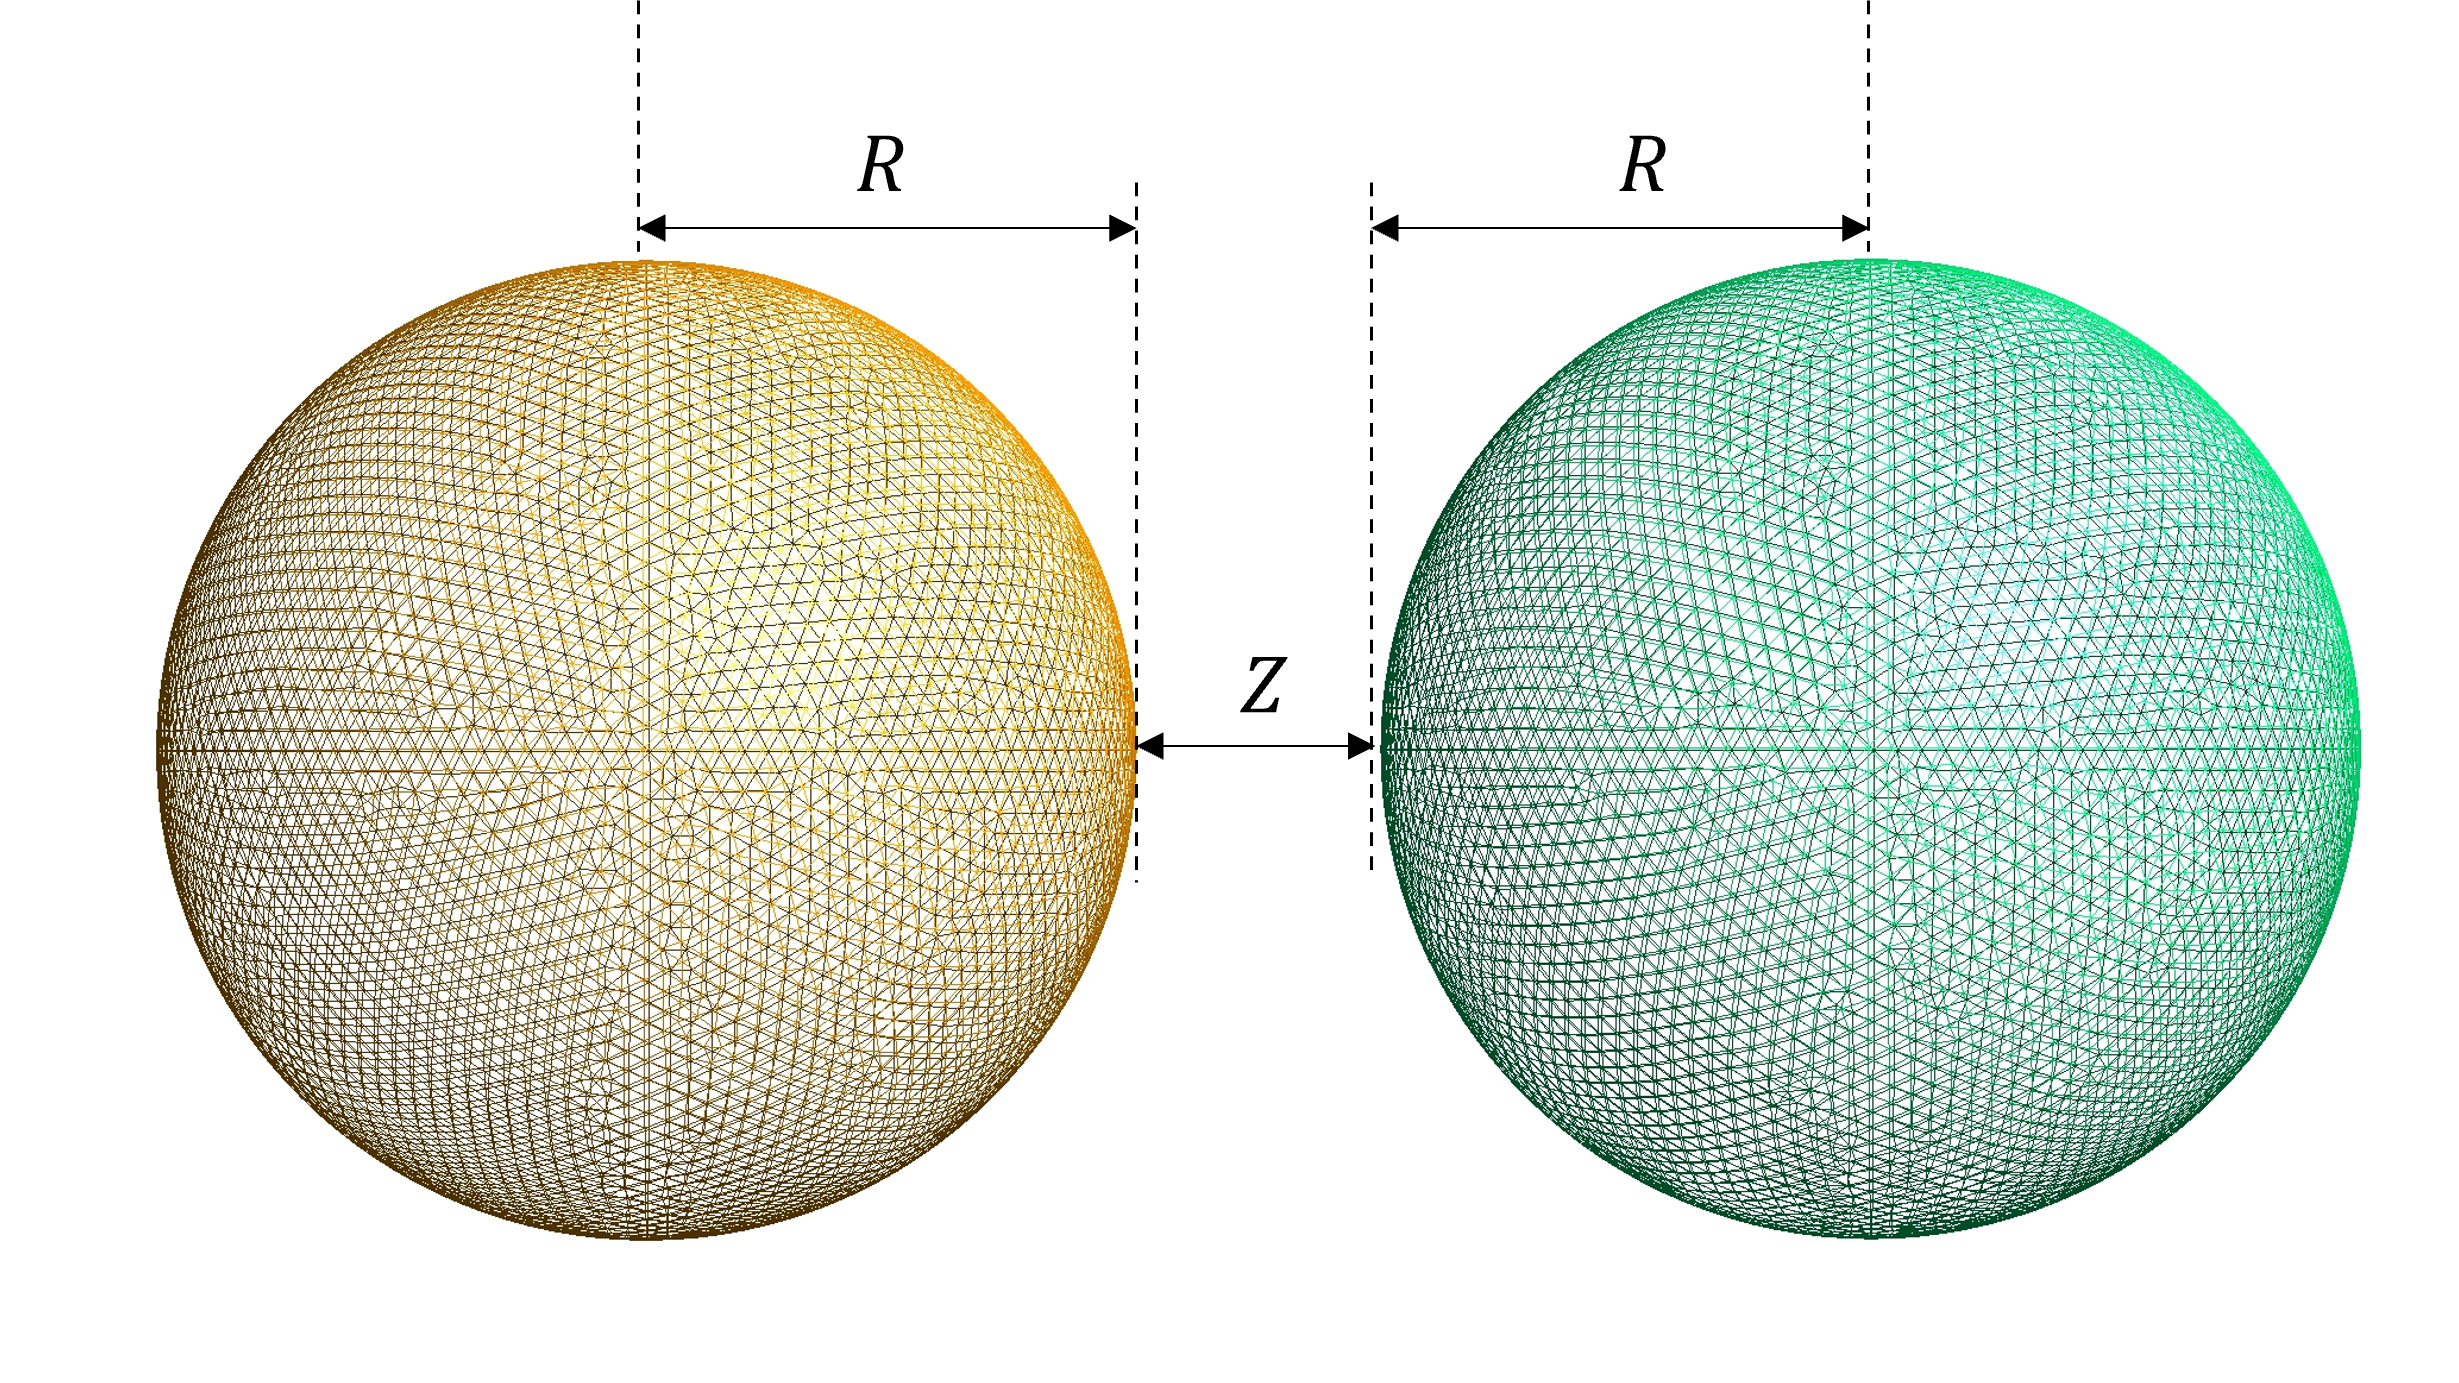
\includegraphics[scale = 0.6]{figures/Grid_two_spheres_dist.png}
    \caption{Two spheres with equal radii: $R$ represents the radius of the spheres and $Z$ is the distance between them.}
    \label{Two spheres with equal radii}
\end{figure}

\begin{figure}[H]
    \includegraphics[scale = 0.7]{figures/rel_dist_equal_radii.pdf}
    \caption{Relative distance between the reference value (computed by Richardson extrapolation) with the asymptotic series, the estimates evaluated when the 
    grid size $h = 0.05$ and 0.1, the estimates evaluated by the standard Arnoldi method and inverse-free Krylov subspace method.
     {\color{red}{should add inverse-free Krylov method later on the figure}}}
    \label{equal_radii_rel_dist}
\end{figure}

From the Figure \ref{equal_radii_rel_dist}, when the grid size $h$ decreases from 0.1 to 0.05, the relative distance between the exact value of the Casimir energy and the estimates 
goes down as well. Since the asymptotic expansion of the Casimir energy only works when the distance between two spheres is asymptotically large, the relative 
distance between the exact value and the asymptotic one decreases as we increase the distance between the spheres. In addition, we apply the standard Arnoldi
method to efficiently compute the Casimir energy and set the dimension of the Krylov subspace inside the algorithm as $m = 20$ and $50$ and we can easily find 
as we increase the Krylov subspace dimension, the relative distance decreases.

\begin{figure}[H]
    \hspace*{2cm}\includegraphics[scale = 0.6]{figures/Grid_two_spheres_unequal_radii.png}
    \caption{Two spheres with unequal radii: $R_{1}$ and $R_{2}$ represent the radius of the spheres and $Z$ is the distance between them.}
    \label{Two spheres with unequal radii}
\end{figure}

When the perfectly conducting spheres have different radii (see Figure \ref{Two spheres with unequal radii}), $R_{1}$ and $R_{2}$ and the centre distance 
is $L = 2R+Z$, then the asymptotic expansion of the Casimir energy at asymptotically large distance can be written as:
\begin{align}\label{Asymptotic unequal radii}
    \mathcal{E} = -\frac{\hbar c}{\pi}\frac{1}{L}\sum_{n=0}^{\infty}\tilde{b}_{n}(\eta)\left(\frac{R_{1}}{L}\right)^{n+2},
\end{align}
where the coefficients $\{\tilde{b}_{n}\}$ depend on the parameter $\eta = R_{2}/R_{1}$ and the first six coefficients are
\begin{align*}
    \tilde{b}_{0} &= -\frac{\eta}{4}, \ \ \ \ \ \tilde{b}_{1} = -\frac{\eta + \eta^{2}}{8}, \ \ \ \ \  \tilde{b}_{2} = -\frac{34(\eta+\eta^{3})+ 9\eta^{2}}{48}, \ \ \ \ \ \tilde{b}_{3} = -\frac{2(\eta+\eta^{4}) + 23(\eta^{2} + \eta^{3})}{32}, \\ 
    \tilde{b}_{4} &= -\frac{8352(\eta + \eta^{5})+ 1995(\eta^{2} + \eta^{4}) + 38980\eta^{3}}{5760}, \ \ \ \ \ \tilde{b}_{5} = -\frac{-1344(\eta+\eta^{6}) + 5478(\eta^{2} + \eta^{5})+2357(\eta^{3} + \eta^{4})}{2304}.
\end{align*}
({\color {red}{Add relative distance figure for unequal radii case }} )

\subsection{Realistic objects case}
{\color {blue} The scatterers are set as some realistic objects (or something complex such as 8-branch ice crystal) and we compute the Casimir energy between them 
in the scalar case.} 


\section{Conclusion}\label{Conclusion}
We have introduced the representation of the Casimir energy in terms of the boundary integral operators and its connection to the relative Krein spectral shift 
function. With the rigorous proof of the Casimir energy formula, we present several numerical methods for 
the calculation of the Casimir energy by applying the spectral properties of the Galerkin discretized form of the boundary 
integral operators. These methods are based on the classical Krylov subspace projection methods and subspaces recycled also significantly reduce the number of the matrix-vector 
multiplications and speed up the calculations for large-scale practical problems. 

For the future work, we will consider the calculation of the Casimir energy in electromagnetic scattering and apply the fast multipole method (FMM) 
when assembling the boundary operator with a shorter assembly time but slower matvecs and compare with the method without implementing FMM.

%\section{Bibliography styles}
% \cite{Feynman1963118}.

% \section*{References}

\bibliography{mybibfile_}

\end{document}